\documentclass[11pt]{report}
\usepackage[margin=2.5cm]{geometry}
\usepackage[french]{babel}
\usepackage[T1]{fontenc}
\usepackage[explicit]{titlesec}
\usepackage{times}
\usepackage{fancyhdr}
\usepackage{graphicx}
\usepackage{ucs}
\usepackage[utf8x]{inputenc}
\usepackage{awesomebox}
\usepackage{fontawesome5}
\usepackage{hyperref}
\setmainfont{Liberation Serif}

\titleformat{\chapter}[display]{\Huge}{\thechapter. #1}{20pt}{\small}

\titlespacing{\chapter}{0pt}{.1cm}{.1cm}

\lhead[\rightmark]{\rightmark}
\chead[]{}
\rhead[\thepage]{\thepage}

\lfoot[]{}
\cfoot[\thepage]{\thepage}
\rfoot[]{}

\renewcommand{\headrulewidth}{0.5pt}

\pagestyle{fancy}

\begin{document}
\begin{titlepage}
   \begin{center}
       \vspace*{5cm}

       \Huge\textbf{Manuel utilisateur}

       \vspace{0.5cm}
       \Large


       Moteur 3D - 7Physics


       
\includegraphics[width=2cm]{./logo.png}

       \vspace{1cm}

       \large
       \textbf{Équipe 3 : Noa AMMIRATI, Fanny DELNONDEDIEU, Quentin GENDARME, Pierre LOTTE, Théo PIROUELLE, Éléa TURC}

       \vfill

       
\includegraphics[width=15cm]{./enseeiht.jpeg}

       \vspace{2cm}

       ENSEEIHT\\
       Département Sciences du Numérique\\
       1APP SN 2020-2021


   \end{center}
\end{titlepage}


\tableofcontents


\chapter{Introduction}

L'idée de ce projet est de réaliser un moteur 3D permettant de réaliser des simulations de notions de physique élémentaires telles que la gravité, les collisions, etc.\newline

Ce projet pourrait alors se séparer en 2 objectifs principaux qui sont aussi les 2 briques principales nécessaire à sa réalisation :\newline

\begin{itemize}
  \item Créer une bibliothèque de rendu des formes tri-dimensionnelles basiques telles que des cubes, sphères, pyramides, etc. Tout cela avec possibilité de changer le point de vue de l'utilisateur en se déplaçant dans l'espace (concept de caméra à la première personne). Ajouté à cela, il est possible de créer plusieurs fonctionnalités visuelles telles que la présence d'ombre et de lumière, de texture, etc. Afin de créer des objets 3D réalistes.\newline

  \item Créer un moteur physique responsable de la simulation des concepts évoqués plus tôt (gravité, collisions, etc.). Tous ces concepts pourront alors être manipulés à souhait grâce à des notions de vélocité, de poids, etc. Qui sont autant de paramètre influant sur ces phénomènes physiques.\newline
\end{itemize}


\chapter{Principales fonctionnalités}

\section{Sprint 0}

Puisque nous avions du temps après la mise en place du projet, nous avons pu
mettre en place des fonctionnalités basiques permettant la compréhension
de ce que nous allions développé par la suite. Nous avons donc cherché à pouvoir nous repérer dans l'espace.

\subsection{Affichage d'une scène 3D}

Une des premières fonctionnalités à implanter a été la création d'une scène 3D. 
Cette scène 3D est constituée d'un sol représentant une grille blanche sur fond gris et d'un ciel bleu.
Cette scène a pour but de permettre à l'utilisateur de mieux comprendre l'orientation des objets,le placement
de sa caméra, etc. Cela permettra alors, lors de simulation physiques, de mieux comprendre les résultats de celles-ci.

\awesomebox{\faCheckCircle}{3pt}{green}{Cette fonctionalité a été complètement réalisée durant cette itération.}

\subsection{Manipulation de la caméra}

Par la suite, et dans l'objectif de pouvoir observer la scène sous plusieurs angles, nous avons implanté une première
version de gestion de la caméra. Grâce à cela, il nous était alors possible de nous déplacer dans la scène grâce
aux raccourcis clavier que nous avions définis.

\awesomebox{\faCheckCircle}{3pt}{green}{Cette fonctionalité a été complètement réalisée durant cette itération.}

\section{Sprint 1}

L'objectif du sprint 1 a été de fournir une première version de l'interface utilisateur lui permettant
d'ajouter des formes 3D prédéfinies à la scène et de les visualiser sous différents angles facilement et intuitivement.

\subsection{Ajout d'un objet 3D}

Tout d'abord, nous avons rendu possible l'ajout de 2 formes prédéfinies que sont le cube et la sphère.

\awesomebox{\faCheckCircle}{3pt}{green}{Cette fonctionalité a été complètement réalisée durant cette itération.}

\subsection{Amélioration de la caméra}

Nous nous sommes aperçus que les raccourcis claviers mis en place lors du sprint 0 étaient difficilement utilisables.
De plus, la première version ne consistait pas vraiment à faire bouger la caméra mais plutôt à faire tourner la scène
sur elle-même. Nous avons donc décidé de changer de manière d'implanter la fonctionnalité et de permettre par la même
occasion l'utilisation de la souris pour une meilleure expérience utilisateur.

\awesomebox{\faCheckCircle}{3pt}{green}{Cette fonctionalité a été complètement réalisée durant cette itération.}

\subsection{Création de l'interface graphique}

Afin de pouvoir une première version utilisable de notre application, nous avons créé, avec l'appui d'une maquette
créée lors du Sprint 0, la base de l'interface utilisateur. Pour commencer, nous avons mis en place la structure de la
fenêtre. Puis, nous avons ajouté les composants nécessaire à l'utilisation des fonctionnalités développées jusqu'ici.
La scène 3D a donc pu être intégrée à la fenêtre et des boutons et formulaires ont été ajoutés pour que l'utilisateur
puisse facilement ajouter des formes ou manipuler la caméra.

\awesomebox{\faCheckCircle}{3pt}{green}{Cette fonctionalité a été complètement réalisée durant cette itération.}

\section{Sprint 2}

L'objectif de ce sprint a été de faire bouger les objets en ajoutant les fonctionnalités liées au moteur physique. Pour cela, nous avons modéliser les concepts de force, d'objets et de monde physique.

\subsection{Création des principes de base du moteur 3D}

Afin de compléter les fonctionnalités voulues de notre projet, nous avons commencé à mettre en place les briques
nécessaires à la simulation de la physique. Pour cela, nous avons modélisé le concept d'objet physique. Ce concept
a pour but de représenter la physique d'une forme. Nous avons donc utilisé ce concept pour calculer la position
d'un objet a tout moment d'une simulation ainsi que sa vitesse à partir de toutes les forces qui lui sont appliquées.
Pour cela nous avons utilisé les équations de cinématique suivantes.

\[
      x(t) = x_{0} + v_{0} . t + \frac{1}{2}.a.t^{2}
\]
\[
      v(t) = v_{0} + a.t
\]

Grâce à ces équations et en mesurant le temps qui s'écoule au lancement d'une simulation, nous avons réussi à déplacer
la position de tous les objets 3D en fonction du temps. Puisque nous réaffichons fréquemment les objets et que les calculs sont réalisés
à partir de la position de l'objet, les objets peuvent désormais se déplacer selon les forces appliquées.\newline

\awesomebox{\faCheckCircle}{3pt}{green}{Cette fonctionalité a été complètement réalisée durant cette itération.}

\subsection{Ajout d'une possibilité de sélection des objets}

Afin de manipuler les objets plus facilement, nous avons ajouté, dans l'interface, une liste de boutons. Chacun de ces boutons est lié à un objet et nous permet de le sélectionner pour ensuite le manipuler. L'affichage ainsi réalisé est le suivant:

% Ajouter la photo

Puisque nous pouvons désormais sélectionner une table, il nous faut désormais rendre l'ajout des forces à un objet donné possible.

\awesomebox{\faCheckCircle}{3pt}{green}{Cette fonctionalité a été complètement réalisée durant cette itération.}

\subsection{Manipulation des forces dans l'interface graphique}

Nous avons donc cherché à rendre la manipulation de forces (création et suppression notamment) possible depuis l'interface graphique de notre application. Ainsi, une fois l'objet sélectionné grâce à la fonctionnalité du point précédent, nous affichons les détails de la forme dans l'interface avec la possibilité d'ajouter une force sur l'objet sélectionné. Toutes les forces sont affichées et elles-mêmes sélectionnables, nous avons donc rajouté un bouton permettant la suppression de la force actuellement sélectionné.

\awesomebox{\faCheckCircle}{3pt}{green}{Cette fonctionalité a été complètement réalisée durant cette itération.}

\subsection{Possibilité de lancer la simulation}

Pour finir, toujours dans le but de permettre aux objets de se déplacer, nous avons ajouté un bouton permettant de lancer la simulation.
Une fois ce bouton pressé, nous demandons 60 fois par secondes à tous les objets physiques de mettre leurs positions à jour.

\awesomebox{\faCheckCircle}{3pt}{green}{Cette fonctionalité a été complètement réalisée durant cette itération.}

\section{Sprint 3}

L'objectif de ce dernier sprint a été de finaliser le projet en ajoutant les dernières fonctionnalités réalisables dans le temps imparti : l'ajout de nouvelles formes prédéfinies, la prévisualisation d'un objet 3D, l'importation et l'exportation d'un projet \textit{*.obj} et la détection de collisions. 

\subsection{Ajout de nouvelles formes prédéfinies}
Afin de proposer à l'utilisateur un panel un peu plus large de formes 3D, l'ajout de nouvelles formes a été réalisé.
En plus du cube et de la sphère, il est maintenant possible d'ajouter une pyramide (à base carré ou triangulaire), un cône et un cylindre à la scène 3D.

\awesomebox{\faCheckCircle}{3pt}{green}{Cette fonctionalité a été complètement réalisée durant cette itération.}

\subsection{Prévisualisation d'un objet 3D}
Nous avons ensuite voulu enrichir l'expérience utilisateur en mettant en place la prévisualisation d'un objet 3D avant de valider l'ajout ou non de l'objet à la scène.

\awesomebox{\faCheckCircle}{3pt}{green}{Cette fonctionalité a été complètement réalisée durant cette itération.}

\subsection{Importation et exportation d'un projet \textit{*.obj}}
En prenant en compte toutes les fonctionnalités précédentes, le choix des formes était donc restreint aux formes prédéfinies présentes sur l'interface. Afin d'accroître le champ des possibles, nous avons ajouter la possibilité d'importer un projet \textit{*.obj}. Grâce à cette fonctionnalité, l'utilisateur a plus de liberté et peut ajouter de nouvelles formes qu'il a préalablement créé dans un logiciel de modélisation 3D.\newline

Nous avons ensuite implanter la possibilité d'exporter un projet \textit{*.obj}. L'utilisateur peut donc à tout moment sauvegarder sont projet afin de le récupérer et de continuer ses expérimentations plus tard.

\awesomebox{\faCheckCircle}{3pt}{green}{Cette fonctionalité a été complètement réalisée durant cette itération.}

\subsection{Détection des collisions}
Une fonctionnalité importante d'un moteur 3D est la détection des collisions. Des recherches ont été éffectuées mais la complexité de cette fonctionnalité ne nous a pas permis de réaliser une version complètement finalisée et stable. Toutefois, une première version expérimentale a été implantée.

\warningbox{Cette fonctionalité n'a pas pu être complètement finalisée. Une première version est cependant proposée à l'utilisateur (cf.Manuel utilisateur).}


\chapter{Découpage de l'application}

\hypertarget{découpage}{Afin} de séparer les rôles le plus possibles et permettre l'utilisation, à termes, de parties de l'application
indépendamment, nous avons commencer par créer 4 répertoires git différent. Cela permet alors de n'utiliser que
les fonctions de rendus dans une librairie minimaliste si besoin et de même pour la partie simulation physique.\newline

Dans chaque répertoire était alors développée une des 4 briques de l'application finale:\newline

\begin{itemize}
  \item \textbf{7Physics}: Répertoire contenant le code de l'interface graphique. Ce répertoire se base sur les 3 autres
        et contient l'exécutable final. Son seul rôle est d'articuler les différentes fonctionnalités du moteur et ce
        dans une interface graphique agréable à utiliser.\newline
  \item\textbf{Common}: Répertoire contenant tout le code commun est nécessaire au fonctionnement des autres. Dans ce
        répertoire, nous pouvons trouver la représentation des formes, la définition d'une classe représentant la position,
        un logger permettant de tracer les appels systèmes, etc.\newline
  \item \textbf{Renderer}: Répertoire contenant uniquement les interactions avec le contexte OpenGL. Afin de fonctionner,
        ce répertoire ne nécessite que l'utilisation du répertoire Common. Il est alors tout à fait pensable de n'utiliser
        que cette partie de l'application et de lui demander de fournir un affichage en 3 dimensions à partir de classes
        créées par l'utilisateur.\newline
  \item \textbf{Engine}: Répertoire permettant la simulation physique. Ce répertoire ne nécessite que l'utilsiation
        de Common pour fonctionner. En effet, tout comme Renderer, il est tout à fait pensable de n'utiliser que ce répertoire
        comme une librairie de calcul physique simple.\newline
\end{itemize}

\chapter{Architecture de l'application}

\begin{center}
  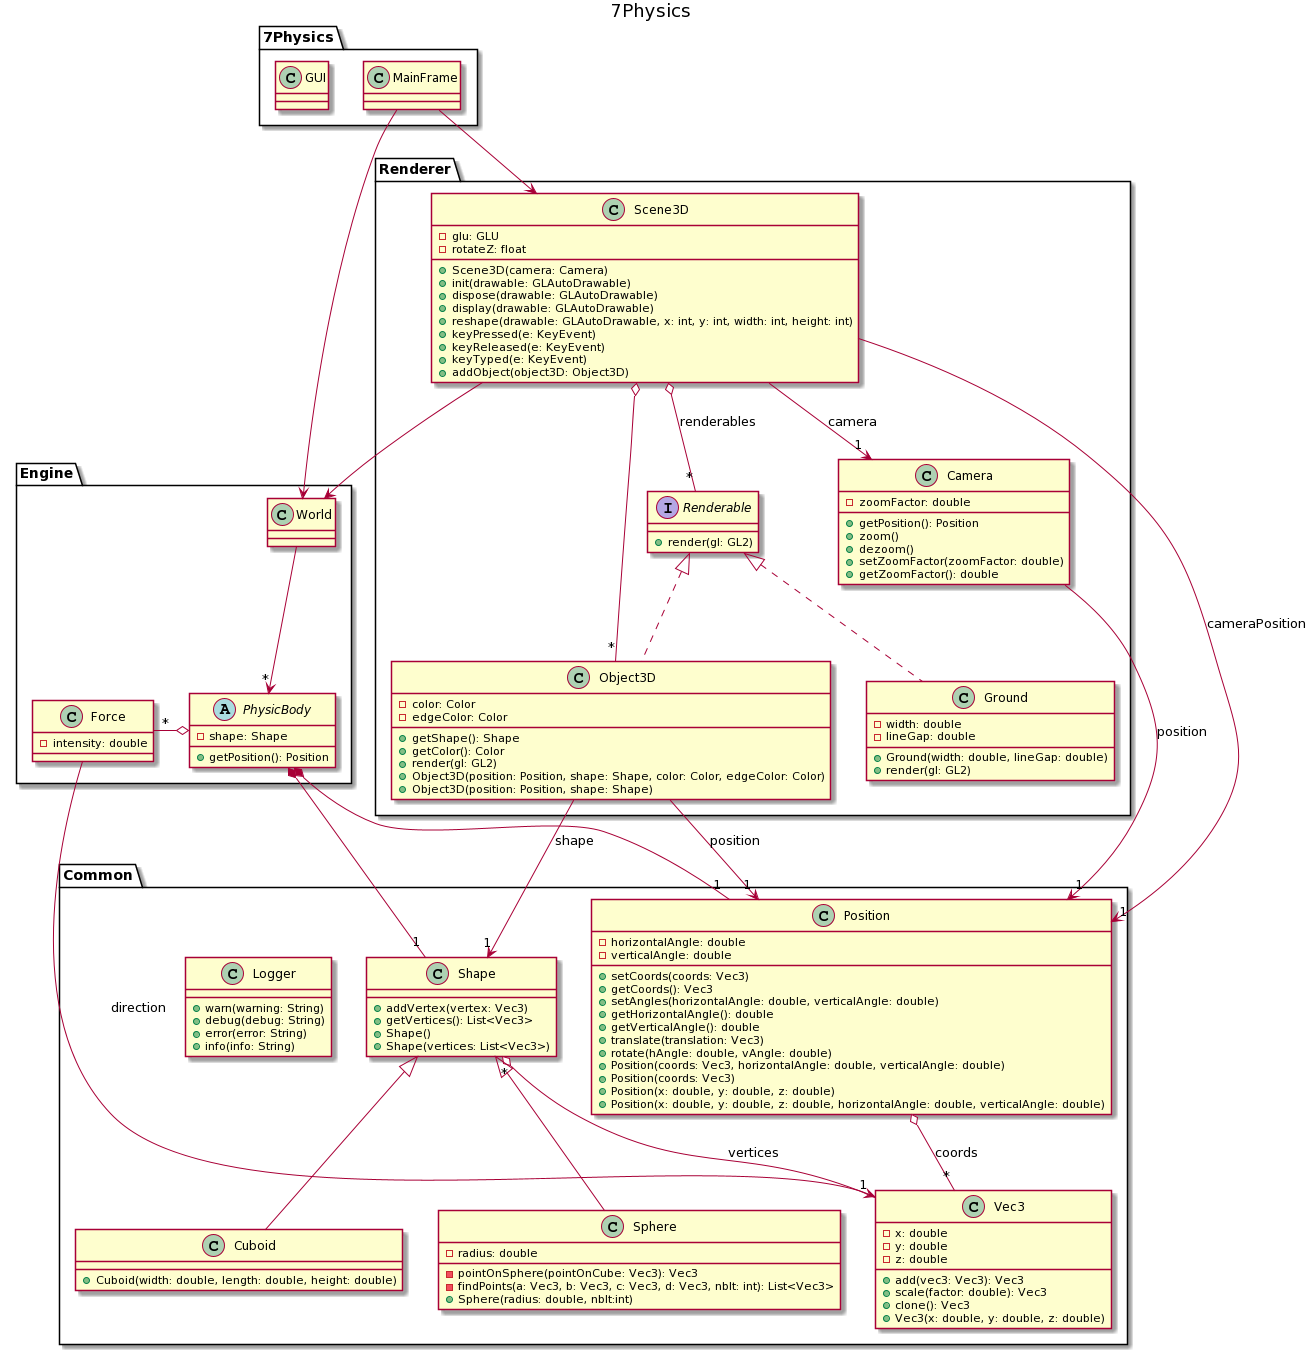
\includegraphics[width=18cm]{./diagramme_classe.png}
\end{center}

\section{7Physics}

Ce répertoire est composé de deux packages : \textit{gui} et \textit{file} ainsi que de la classe \textit{Main.java} permettant de lancer l'application.

\subsection{GUI}
Dans ce répertoire, on retrouve le package \textit{gui} composé de la classe \textit{GUI.java} qui représente la fenêtre principale de l'application. Elle hérite donc de \textit{JFrame}, le composant \textit{SWING} permettant la création d'une fenêtre principale avec une bordure et une barre de titre.

C'est donc dans cette classe que l'interface principale est définie avec les différents conteneurs (\textit{JPanel}, \textit{JMenu}) contenant d'autres composants (\textit{JButton}, \textit{ImageIcon}, \textit{JMenuItem}, ...).

Dans cette classe, le patron de conception \textit{Singleton} a été implanté. En effet, nous souhaitions nous assurer qu'une seule fenêtre principale ne puisse exister et donc qu'un unique point d'accès soit possible.

Afin de séparer le code, certains composants ont été séparés de la classe \textit{GUI}. Les différents \textit{JPanel} utilisés pour l'ajout des formes prédéfinies ont été créés dans des classes séparées. De même concernant certains \textit{ActionListener}, les interfaces "auditrices" pour différents types d'évènements à traiter.


\subsection{Files}
Dans ce même répertoire, on retrouve aussi le package \textit{file}. Ce package contient la classe \textit{OBJFile.java} qui permet de manipuler des fichiers \textit{*.obj}. Elle permet de fournir une méthode permettant d'extraire le contenu d'un fichier \textit{*.obj} et de faire le traitement nécessaire afin de fournir les formes à afficher à la scène 3D.
Elle permet aussi la création d'un fichier \textit{*.obj} à partir du contenu de la scène 3D courante.

\subsection{Tests}

Une classe de test a été réalisée afin de tester la classe \textit{OBJFile} avec différents fichiers \textit{*.obj} (taille et contenu différent).

\section{Common}
Le répertoire \textit{Common} est composé de deux packages : \textit{logger} et \textit{geom}.

\subsection{Logger}
Dans le package \textit{logger}, la classe \textit{Logger} représente la classe utilitaire gérant les logs du projet.

\subsection{Types utilitaires}
Dans le package \textit{geom}, il y a différentes classes définissant des types utilitaires. Nous avons par exemple, la classe \textit{Vec3} qui représente un vecteur à trois dimensions, la classe \textit{Position} représentant une position et la classe \textit{Shape} représentant une forme en trois dimensions.

\subsection{Formes prédéfinies}
Dans le package \textit{geom}, nous avons un nouveau package \textit{shape} représentant les différentes formes prédéfinies tels que le cone, le cube, la pyramide, la sphere, ...

\subsection{Tests}
Une classe de test a été réalisée afin de tester avec différents formes 3D (cube et sphère), la classe \textit{BoundingBox} qui représente les bordures des objets 3D.

\section{Engine}
Ce répertoire est composé de plusieurs classes : \textit{PhysicObject}, \textit{World}.

\subsection{PhysicObject}
La classe \textit{PhysicObject} représente un objet 3D dans l'environnement ayant des caractéristiques physiques.

Un \textit{PhysicObject} est créé à partir d'une \textit{Shape}, d'une \textit{Position} et d'une vitesse initiale.
Nous pouvons lui ajouter/supprimer des forces, mettre à jour sa position et sa vitesse en fonction des forces appliquées.

\subsection{World}
La classe \textit{World} représente un monde 3D avec un sol d'une certaine dimension. Il est possible d'ajouter un \textit{PhysicObject}, d'appliquer la gravité au monde 3D, de gérer les collisions.

\subsection{Tests}
Deux classes de test ont été définies : \textit{TestCollisions}, \textit{TestPhysicBody} afin de vérifier l'effet des collisions et les résultats obtenus après application de plusieurs forces sur un \textit{PhysicObjetc}, . 

\section{Renderer}
Ce dernier répertoire est composé d'éléments permettant le rendu graphique 3D.

\subsection{Camera}

\subsection{Object3D}

\subsection{Scene3D}

\subsection{Ground}

\subsection{Tests}
Des tests graphiques ont été réalisés afin de vérifier visuellement la suppresion d'un objet de la scène par exemple.

\subsection{Interaction avec OpenGL}

\chapter{Principaux choix}

\section{Conception}

\subsection{Création de la maquette IHM}

A l'aide de l'outil Figma, une maquette de l'interface graphique a été réalisée afin de concrétiser les idées des membres de l'équipe
et de représenter concrètement le logiciel à construire. Nous avons choisi ce logiciel de design car il offrait la possibilité de
collaborer sur un projet unique. En apportant tous nos avis sur cette maquette, nous avons pu obtenir une representation réaliste qui à
été utile lors du développement de l'IHM.

\subsection{Création d'un diagramme de classe}

Après avoir défini les besoins auxquelles notre application devra répondre, nous avons réfléchi au découpage du projet \hyperlink{découpage}{(voir Découpage de l'application)}.
A partir de ce découpage, nous avons créer un diagramme de classe initial qui nous a servi de base à nos développements. 
Au fur et à mesure de l'affinement de nos visions sur chaque partie de l'application nous avons adapté le diagramme de classe en conséquence.
Nous avons utilisé l'outil plantuml pour créer ce diagramme ce qui nous a permis de ne pas perdre du temps de mise en page. 

\section{Réalisation}

\section{Problèmes rencontrés et solutions apportées}

\subsection{Rafraîchissement du rendu graphique}

Lors de la première version de notre projet, la caméra avait un déplacement sacadé rendant l'expérience utilisateur médiocre. Nous avons alors
cherché à régler ce problème en augmentant le taux de rafraîchissement de la caméra à 60 images par seconde. De plus, nous avons diminué
les valeurs utilisées pour déplacer la caméra afin de donner plus de contrôle et rendre l'animation plus fluide.

\subsection{Caméra fixée sur la scène}

Nous n'avions, au début du projet pas connaissance de la bonne utilisation et réalisation de la caméra dans un contexte OpenGL. Nous avions
donc commencé par faire tourner la scène sur elle même sans bouger le point de vue. Cela donnait alors la possibilité de voir la scène sous tous les angles mais n'était en aucun cas une bonne utilisation de la caméra. Nous avons fini par trouver une solution dans une des classes fournies par la librairie nous permettant d'utiliser OpenGL. Cela nous a alors permis d'obtenir une réelle caméra augmentant ainsi l'expérience utilisateur car la visualisation était beaucoup plus intuitive.

\newpage

\subsection{Rendu pixelisé}


Lors de l'utilisation d'OpenGL dans sa version brute, nous avons remarqué de gros problèmes de résolutions qui se traduisaient alors
par des lignes d'avantages semblables à des escaliers qu'à de vraies lignes droites. Pour corriger cette effet, nous avons utilisé l'option
d'anti-aliasing disponible. Cela a alors amélioré le rendu graphique des objets et de la scène en général.

\subsection{Problèmes de simulation}

Lorsque nous avons ajouté la possibilité d'ajouter des forces sur un objet, nous avons utilisé, afin de calculer la position et la vitesse, des
référentiels de temps absolus. Nous avons donc utilisé, dans nos équations, la position et la vitesse de base et nous avons utilisé comme mesure
de temps, le temps écoulé depuis le début de la simulation. Cependant, cela avait pour effet lors de la modification de forces lors d'une
simulation, de téléporter les objets à la position obtenue si la force avait été présente depuis le début de la simulation.

\chapter{Organisation de l'équipe et mise en oeuvre des méthodes agiles}

\section{Mise en place du projet}
L'objectif du sprint 0 à été de mettre en place le projet. Pour cela, il a tout d'abord fallu
déterminer les différents objectifs et les différents besoins utilisateur au travers de User stories. Ensuite, l'équipe a défini
les outils à utiliser concernant la gestion de projet, la gestion du code et la communication au sein de l'équipe.
Pour finir, le projet a été structuré en différents répertoires au sein de l'organisation GitHub créée pour le projet long
et l'environnement de travail a été configuré pour chaque membre de l'équipe.\newline

Une fois cela fait, nous avons pu commencer à réaliser les premières User Stories.

\section{Utilisation des cérémonies agiles}

Lors du déroulement du projet, nous avons mis en place 4 types de cérémonies des méthodes agiles.

\subsection{Sprint planning}

Au début de chaque sprint nous avons commencé par se réunir tous ensemble pour faire un point sur l'état d'esprit de tout le monde.
Nous échangions alors sur le ressenti par rapport au projet et l'état d'avancement de celui-ci ainsi que les difficultés eprouvées. Cette première étape
nous permettait alors de s'assurer de la bonne entente entre les membres de l'équipe.

Une fois cela fait, nous continuions par choisir les prochaines User Stories à implémenter au sein de l'application en se basant sur la vélocité
de l'équipe lors du sprint précédent.\newline

Le sprint était alors prêt à commencer.

\subsection{Daily scrum}

Lors du déroulement de chaque Sprint, nous avions des réunions régulières. N'ayant pas forcément le temps
d'avancer chaque jour sur le projet, nous avons donc décidé de nous réunir tous les 2 à 3 jours
pour faire le point sur l'avancement de chacun depuis le dernier daily scrum, les choix de conception et d'implémentation que
nous devions revoir en cours de projet, etc.

\subsection{Sanity Check}

Au milieu de chaque sprint, nous nous réunissions afin de discuter de l'état courant du sprint. Le but était alors, dans le cas
où tout avait déjà été fait, d'ajouter de nouvelles User Stories à réaliser, ou, dans le cas contraire, d'alléger la charge
de travail prévue.

Cette cérémonie nous permettait alors d'être sûr que notre charge de travail était réalisable lors du temps imparti
et de s'assurer que tout se déroulait comme prévu.

\subsection{Sprint Review}

Pour clôturer le sprint, nous organisions une réunion ayant pour but de revenir sur les évènements du sprint.
Cette cérémonie était importante car elle nous permettait notamment de discuter des difficultés rencontrées et calculer la vélocité 
à utiliser lors du prochain sprint planning.

\subsection{Retrospective}

Enfin, l'équipe se réunissait une dernière fois dans le sprint pour analyser le déroulement du sprint. Cette analyse permet d'avoir le ressenti réel de chaque membre de l'équipe sur le projet. Cette réunion faisait ressortir les défauts du sprint réalisé afin de tenter de les corriger lors du prochain.

\end{document}